\chapter{Implementation and evaluation of eGPU}
\label{chap:implementation}

The Section \ref{s:gpusw:nema} discussed on the software implementation in Nema GPU. This chapter discusses the implementation of the algorithm chosen and its results in functionality and run-time performance in the eGPU. The version 7 of the algorithm indicated in the Figure \ref{fig:algover} is used for evaluation purpose. For the purpose of comparison, the algorithm is also implemented in the hardware without the use of eGPU. This would help isolate the performance with and without eGPU. Observations are recorded.
%

%%%%%%%%%%%%%%%%%%%%%%%%%%%%%%%%%%%%%
%%%%%%%%%%%%%%%%%%%%%%%%%%%%%%%%%%%%%
%%%%%%%%%%%%   SECTION   %%%%%%%%%%%%
%%%%%%%%%%%%%%%%%%%%%%%%%%%%%%%%%%%%%
%%%%%%%%%%%%%%%%%%%%%%%%%%%%%%%%%%%%%
\section{Choice of kernels}
\label{sec:kernelchoice}

\begin{figure}
    \center
    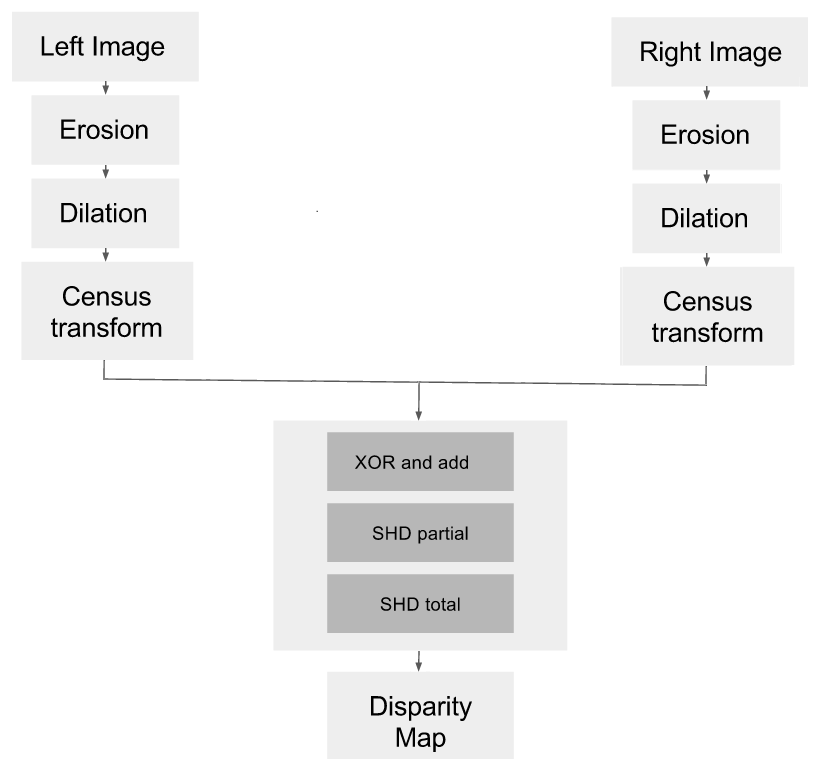
\includegraphics[width=.7\linewidth]{figures/Algorithm}
    \caption{Block diagram of algorithm implemented.}
    \label{fig:algorithm}
\end{figure}

The Figure \ref{fig:algorithm} shows the block diagram of the algorithm implemented. Here all the blocks can take advantage of eGPU parallelization as each of them perform the same operation across all the pixels. Hence, a kernel is written for each of the steps. For the purpose of SHD calculation, three kernels are required. This is due to lack of synchronization facilities between threads as discussed in the Section \ref{s:gpusw:nkernels}. For example, the partial SHD calculation part needs to be performed only after the XOR add step is completed for all the pixels. In Nema, it is not possible to implement both of them in a single kernel as there is no way of determining within a thread if all other threads have completed till certain step of the algorithm. This is a disadvantage as SHD involves loop operation with disparity value as a parameter as explained in the Section \ref{sec:optdmalgo}. This means three kernels need to be loaded for each iteration for XOR add, SHD partial and SHD total respectively. The function was experimented by using a single kernel and using conditional statements to decide on the thread functionality. However, this resulted in a slower performance probably due to incorrect branch predictions involved. Hence, a kernel for morphological erosion, morphological dialation, census transform, XOR addition, partial SHD calculation and total SHD calculation were created. This results in multiple kernels getting loaded for each iteration of the DM algorithm discussed in \ref{sec:optdmalgo}.
%

%%%%%%%%%%%%%%%%%%%%%%%%%%%%%%%%%%%%%
%%%%%%%%%%%%%%%%%%%%%%%%%%%%%%%%%%%%%
%%%%%%%%%%%%   SECTION   %%%%%%%%%%%%
%%%%%%%%%%%%%%%%%%%%%%%%%%%%%%%%%%%%%
%%%%%%%%%%%%%%%%%%%%%%%%%%%%%%%%%%%%%
\section{Functional Performance}
\label{sec:fperformance}

% Please add the following required packages to your document preamble:
% \usepackage{booktabs}
\begin{table}[!htbp]
\centering
\begin{tabular}{@{}|c|c|c|@{}}
\toprule
\textbf{Image}  & \textbf{BMPRE Intel Corei3} & \textbf{BMPRE zc706+Nema} \\ \midrule
Tsukuba frame 1 & 54762                       & 54499                     \\ \bottomrule
\end{tabular}
\caption{BMPRE across different hardware including Nema eGPU}
\label{tab:bmprenema}
\end{table}

\begin{figure}
    \center
    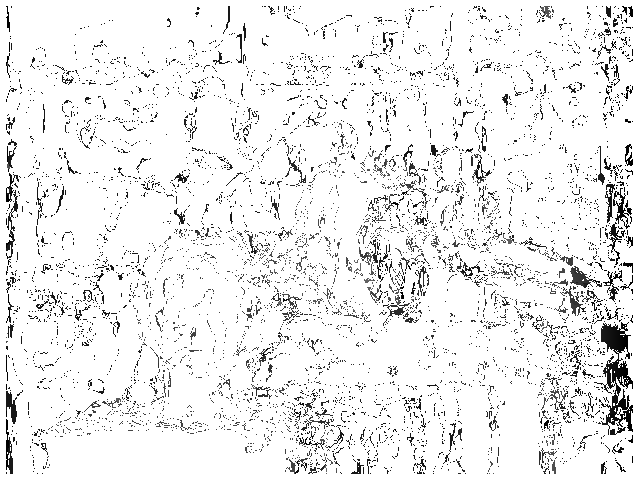
\includegraphics[width=.7\linewidth]{figures/diffpixeGPU}
    \caption{Pixels in eGPU disparity map that are different from Intel Core i3 disparity map.}
    \label{fig:diffpixegpu}
\end{figure}
As discussed in the beginning of this chapter, the algorithm is run with and without the eGPU for the purpose of performance comparison. BMPRE method discussed in the Section \ref{s:stereovision:bmpre} is used for functional evaluation. Ideally, same functional performance as observed in the software implementation is expected while using hardware. The first frame of Tsukuba dataset is used for the functional verification purpose. The Table \ref{tab:bmprenema} shows the BMPRE values in Intel Corei3, zc706 evaluation board with the Nema eGPU. It can be seen that there is a marginal difference in the values across hardwares, with the eGPU performing better. In order to understand the reason behind this, the pixels which are different from the Intel Corei3 result are looked into. The Figure \ref{fig:diffpixegpu} shows the pixels which are different in eGPU implementation from the Intel Core i3 implementation. There is not a particular pattern in the location of these pixels. Hence, the idea of these pixels arising due to synchronization between threads in Intel version of the program can be rejected. Further analysis needs to be done with more image sets to narrow down the reason for the difference.

%%%%%%%%%%%%%%%%%%%%%%%%%%%%%%%%%%%%%
%%%%%%%%%%%%%%%%%%%%%%%%%%%%%%%%%%%%%
%%%%%%%%%%%%   SECTION   %%%%%%%%%%%%
%%%%%%%%%%%%%%%%%%%%%%%%%%%%%%%%%%%%%
%%%%%%%%%%%%%%%%%%%%%%%%%%%%%%%%%%%%%
\section{Execution time}
\label{sec:rtperformance}

% Please add the following required packages to your document preamble:
% \usepackage{booktabs}
\begin{table}[!htbp]
\centering
\begin{tabular}{@{}|l|l|l|l|@{}}
\toprule
\multicolumn{1}{|c|}{\textbf{Hardware}} & \multicolumn{1}{c|}{\textbf{Work time (eGPU)(s)}} & \multicolumn{1}{c|}{\textbf{Work time (host)(s)}} & \textbf{Program execution time(s)} \\ \midrule
Intel core i3                           &                                                        &                                                      & 0.7010273                    \\ \midrule
zc706                                   &                                                        &                                                      & 5.95241                      \\ \midrule
zc706+Nema                              & 32.665                                                 & 39.3129                                              & 40.9769                      \\ \bottomrule
\end{tabular}
\caption{Execution time of algorithm in Nema in comparison with other hardware. The time eGPU is active as measured by the eGPU itself (Work time (eGPU)) and the host processor (Work time (host)) are indicated. Program execution time indicates the total execution time including the image I/O.}
\label{tab:nemart}
\end{table}

In order to gauge the execution time, the algorithm is run in zc706 hardware with and without the Nema GPU. Again frame 1 from the Tsukuba dataset is used for the evaluation. The Table \ref{tab:nemart} shows the difference in execution time of the algorithm across different hardware. The table shows two entries for work time of the Nema eGPU. Worktime (host) is measured by the program running on the host processor. It is the difference in time between command list is flushed, and an interrupt indicating Nema operation is complete is raised. Work time (eGPU) is the time Nema cores are active as measured by the internal hardware of eGPU. It can be seen that host indicates a higher time compared to the one indicated by the GPU. This probably means that Nema cores are idle for some time during the execution of threads.

\begin{figure}[!htbp]
\captionsetup{justification=centering}
\captionsetup[subfigure]{justification=centering}
\begin{subfigure}{.5\textwidth}
  \centering
  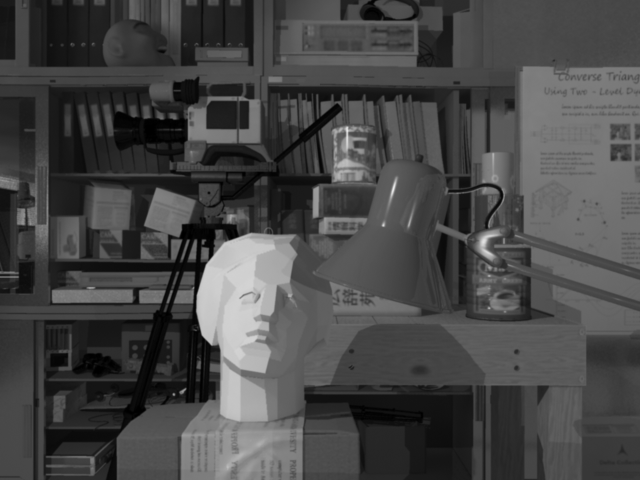
\includegraphics[width=.8\linewidth]{figures/frame_1_monochrome}
  \caption{Monochrome image.}
  \label{fig:sfig1}
\end{subfigure}%
\begin{subfigure}{.5\textwidth}
  \centering
  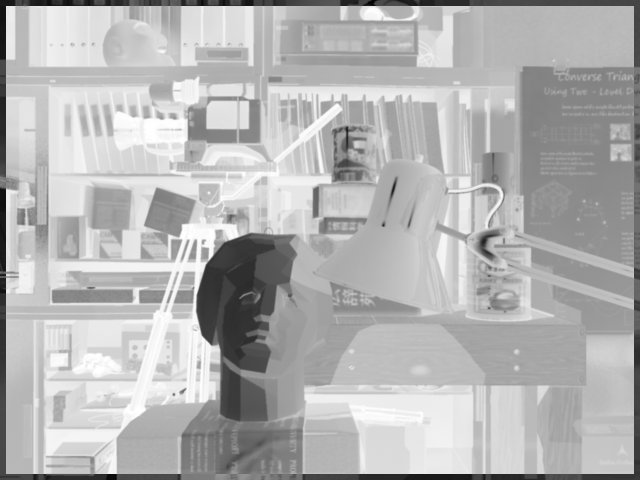
\includegraphics[width=.8\linewidth]{figures/negated}
  \caption{Negated image.}
  \label{fig:sfig2}
\end{subfigure}
\caption{Negation of left camera monochrome image, frame 1, Tsukuba dataset.}
\label{fig:negation}
\end{figure}


The algorithm is seen to run slower with the Nema GPU compared to the case without it. There could be possibly few factors behind this. 
\begin{itemize}
\item{Nema runs at a slower speed(83MHz) compared to the host processor(800MHz). Silicon implementation of Nema will result in a faster performance.}
\item{From the Section \ref{sec:kernelchoice} it can be seen that there are three kernels loaded for each iteration of the program. It might be possible that the kernel loading time is much higher than the actual execution time. However Work time (eGPU) from the Table \ref{tab:nemart} suggests that execution time is higher. As a sanity check a simpler program with a single kernel, loaded only once is evaluated at runtime. The program performs negation of pixels as shown in the Figure \ref{fig:negation}.The results are as shown in the first row of the Table \ref{tab:nemartneg}. This confirms that loading of kernels is not the prime factor influencing the slower run-time.}
\item{The slowdown could be a result of poor hardware thread management. Since Nema has only 4 cores with 16 threads each, only 64 threads can run at a time. A software thread management experiment was done by programatically deploying 64 threads at a time, and waiting for them to complete before deploying the next 64 threads and so on. This was done for the negate program to find out if the eGPU's hardware thread management was slowing the system down. However, this turned out not to be true as shown in the second row of the Table \ref{tab:nemartneg}. Note that the Nema working time as measured by the eGPU itself is shown as zero as each set of threads complete within a span of a ms, thus being too fast to measure.}
\item{Nema has a common data cache of 1MB for all the four cores. Each core runs independently of the others, so each core most likely executes a different part of the kernel. Since cores can operate on different data points along the image, there might be data conflict between the cores leading to high miss rates. This cannot be confirmed as currently Nema does not keep track of cache statistics.}

\end{itemize}

% Please add the following required packages to your document preamble:
% \usepackage{booktabs}
\begin{table}[!htbp]
\centering
\begin{tabular}{@{}|c|c|c|c|@{}}
\toprule
\textbf{Program}                  & \textbf{Work time (eGPU)(s)} & \textbf{Work time (host)(s)} & \textbf{Program run time(s)} \\ \midrule
Negate & 0.016                             & 0.0351441                       & 0.913559                     \\ \midrule
Negate (software thread management) & 0                                 & 77.3031                         & 78.1798                      \\ \bottomrule
\end{tabular}
\caption{Nema execution time results for the Negate program with and without software thread management.}
\label{tab:nemartneg}
\end{table}